\subsection{Output Analysis of $S(n)$ and $S(d)$}



\subsubsection{Relationship Between $n$ and $d$}


In this section, the displacement of a particle, $d$, is the shortest
distance from the initial to the stop position in the infinite tiling
plane. In theory, the mean square displacement (MSD) of $N$ Brownian
particles at $n-$th step in $2-$dimensional space is defined as

     \begin{equation}\label{eq:mds_N}
       MSD = \langle \lvert \bm{r}(n) \lvert^2 \rangle = \frac{1}{N} \sum^{N}_{i=1} (\bm{s}_{i}(n) - \bm{s}_{i}(0))^2 = 4Dn
     \end{equation}
     
where the subscript, $i$, refers to each particle for which the MSD is
calculated. $\bm{s}_{i}(n)$ and $\bm{s}_{i}(0)$ are the $i-$th
particle positions at $n-$th step and at the initial time,
respectively. $D$ is diffusion coefficient which is related to the
variance of the independent displacements of the particle. In the
simulation, $D$ equals $1$.
     
      
      \begin{figure}
         \centering
         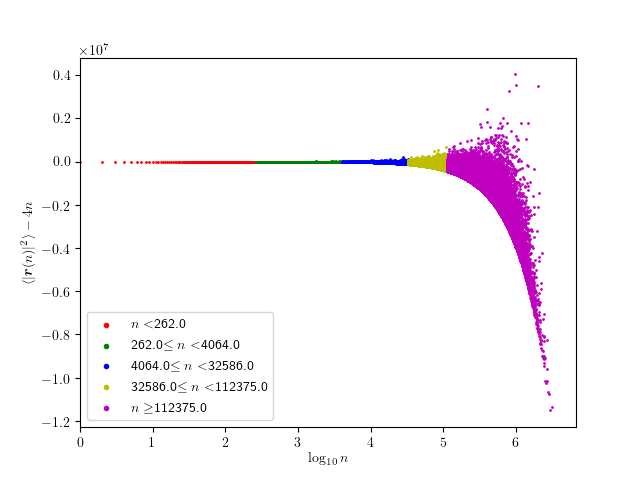
\includegraphics[width=\textwidth]{G_1_L_3_msd_n.png}
         \caption{Particles in $G_1L_3$ are divided into several
           subgroups based on various intervals of steps, and their
           colours are as identical as the segments in
           Fig.~\ref{fig:steps_seg_curve_G_1_L_3}.}
         \label{fig:G_1_L_3_msd_n}
      \end{figure}


Eq.~\ref{eq:mds_N} indicates a linear relationship between the mean
square displacement of the particle and the number of steps. It is a
feature of the normal diffusive behavior. Fig.~\ref{fig:G_1_L_3_msd_n}
shows how the difference between MSD of the particle and $4n$ varying
over $\log_{10}n$ in LRWs. When $n \leq 4064.0$, the variation is not
equal to $0$ with larger fluctuation, which implies that blue, yellow,
and pink particles undergo anomalous diffusion process. In other
words,

     \begin{equation}\label{eq:anomalous_diffusion}
       \langle \lvert \bm{r}(n) \lvert^2 \rangle \propto n^{\gamma}
     \end{equation}
where $\gamma \ne 1$. In Fig.~\ref{fig:steps_seg_curve_G_1_L_3},
negative variation implies $\gamma < 1$ called sub-diffusion process,
while positive value denotes $\gamma > 1$ named super-diffusion.

     
      \begin{figure}
         \centering
         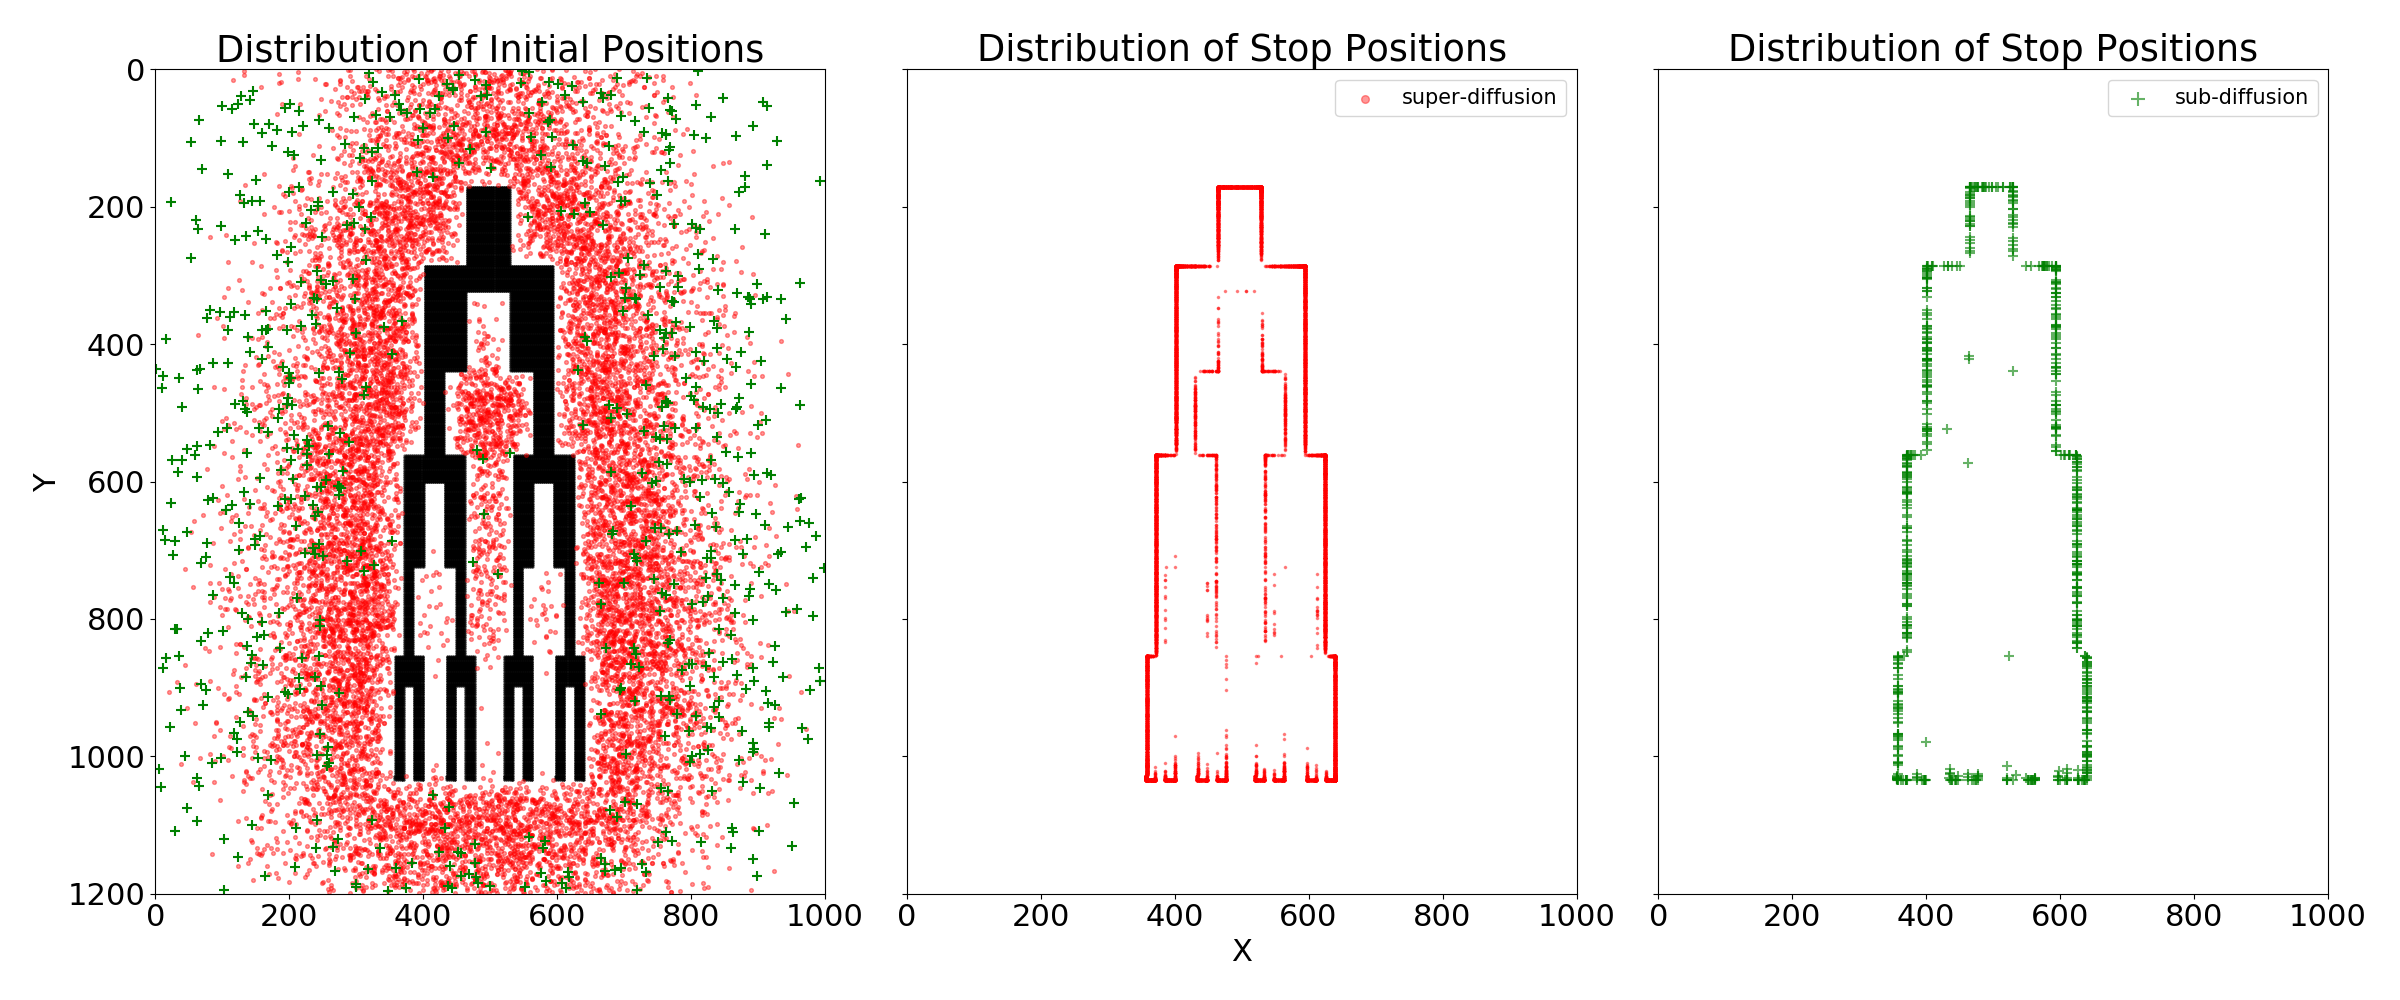
\includegraphics[width=\textwidth]{G_1_L_3_steps_blue_initial_stop_pos_var.png}
         \caption{In the left figure, $696$ dark blue pluses refer to
           super-diffusion particles, which are distributed closer and
           more concentrated to the fringe of the branching
           structure. $15198$ pale blue points represent sub-diffusion
           particles and scatter mainly around the edges of the
           image. In-between the branches, there has only six
           super-diffusion particles and an enormous amount of
           sub-diffusion ones. The middle and right depict the stop
           positions for super and sub-diffusion particles,
           respectively, coloured by a perceptually uniform sequential
           colormap based on their maximum displacement in the tiling
           space.}
         \label{fig:G_1_L_3_var_initial_stop_pos}
      \end{figure}

To understand the underlying mechanism of the anomalous-type diffusion
process, initial and stop positions of particles in
Fig.~\ref{fig:G_1_L_3_steps_blue_initial_pos_distribution}, whose
steps ranged from $4064$ to $32586$, are illustrated in
Fig.~\ref{fig:G_1_L_3_var_initial_stop_pos}. Suppose particles are
trapped in the narrow space in-between the branches or initially start
LRWs near the branching structure. In that case, their movements will
be restricted because of the nearby absorbing boundary condition,
causing the sub-diffusion phenomenon. As shown in the middle subplot
of Fig.~\ref{fig:G_1_L_3_var_initial_stop_pos}, the maximum
displacement of sub-diffusion particles is less than $200$. There also
have exceptional circumstances that $6$ particles, in-between the
limbs, undergo super-diffusion since they can explore a large portion
of space within a predefined range of steps, as shown in the right
subfigure of Fig.~\ref{fig:G_1_L_3_var_initial_stop_pos}. Generally,
particles around the edges of the image will be more likely to pass
through the periodic boundary, reappear in the adjacent cell, and
continue LRWs with the same velocity until hitting the absorbing
boundary, which results in large displacement and the super-diffusion
process.
    

   

\subsubsection{Interpretation of Survival Curves}


   \begin{figure}
        \centering
        \begin{subfigure}[b]{0.45\textwidth}
          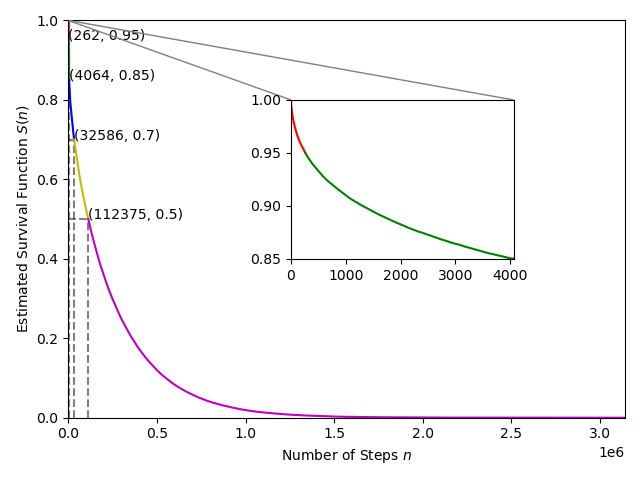
\includegraphics[width=\textwidth]{steps_seg_curve_G_1_L_3.png}
          \caption{}
          \label{fig:steps_seg_curve_G_1_L_3}
        \end{subfigure}
        \hfill
        \begin{subfigure}[b]{0.45\textwidth}
          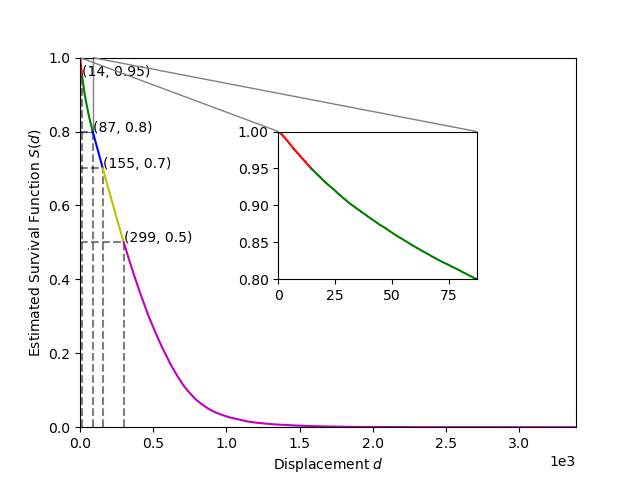
\includegraphics[width=\textwidth]{unwrap_disp_seg_curve_G_1_L_3.png}
          \caption{}
          \label{fig:disp_seg_curve_G_1_L_3}
        \end{subfigure}
        \caption{}
        \label{fig:seg_curve_G_1_L_3_steps_disp}
   \end{figure}



   \begin{figure}
        \centering
        \begin{subfigure}[b]{0.45\textwidth}
          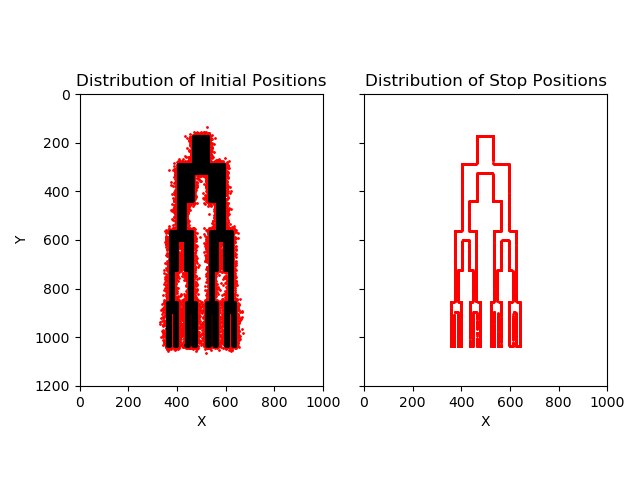
\includegraphics[width=\textwidth]{G_1_L_3_steps_red_initial_pos_distribution.png}
          \caption{}
          \label{fig:G_1_L_3_steps_red_initial_pos_distribution}
        \end{subfigure}
        
        \begin{subfigure}[b]{0.45\textwidth}
          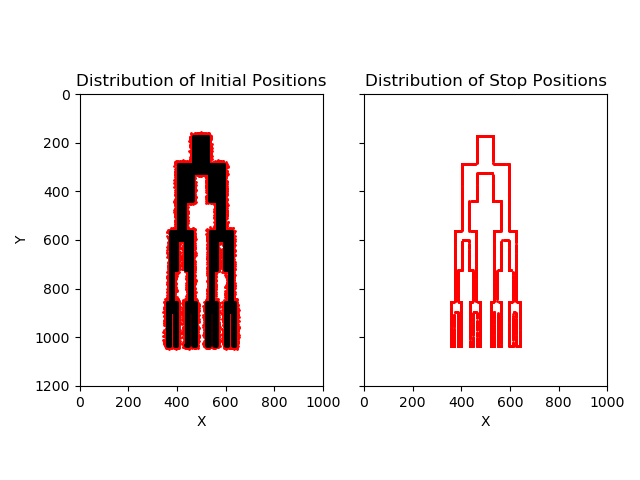
\includegraphics[width=\textwidth]{G_1_L_3_unwrap_disp_red_initial_pos_distribution.png}
          \caption{}
          \label{fig:G_1_L_3_disp_red_initial_pos_distribution}
        \end{subfigure}
        \caption{}
        \label{fig:G_1_L_3_steps_disp_red}
   \end{figure}


   \begin{figure}
        \centering
        \begin{subfigure}[b]{0.45\textwidth}
          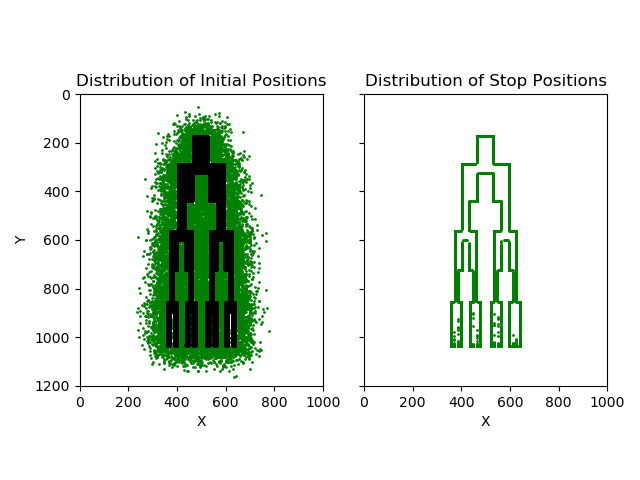
\includegraphics[width=\textwidth]{G_1_L_3_steps_green_initial_pos_distribution.png}
          \caption{}
          \label{fig:G_1_L_3_steps_green_initial_pos_distribution}
        \end{subfigure}
        
        \begin{subfigure}[b]{0.45\textwidth}
          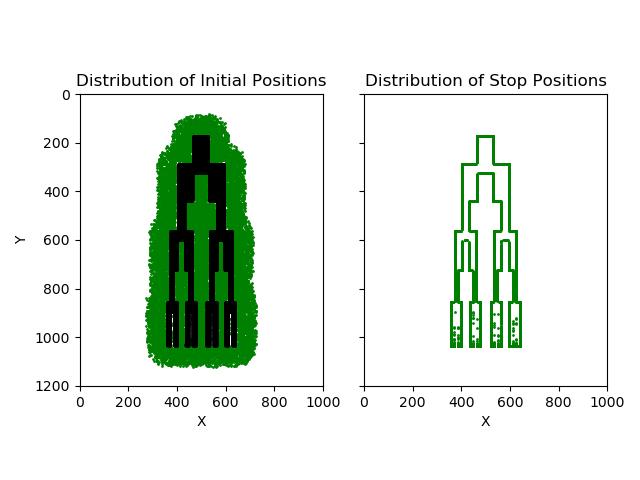
\includegraphics[width=\textwidth]{G_1_L_3_unwrap_disp_green_initial_pos_distribution.png}
          \caption{}
          \label{fig:G_1_L_3_disp_green_initial_pos_distribution}
        \end{subfigure}
        \caption{}
        \label{fig:G_1_L_3_steps_disp_green}
   \end{figure}




   \begin{figure}
        \centering
        \begin{subfigure}[b]{0.45\textwidth}
          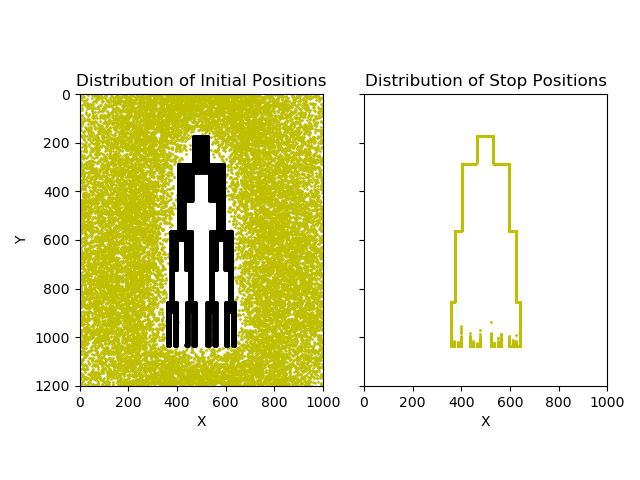
\includegraphics[width=\textwidth]{G_1_L_3_steps_y_initial_pos_distribution.png}
          \caption{}
          \label{fig:G_1_L_3_steps_yellow_initial_pos_distribution}
        \end{subfigure}
        
        \begin{subfigure}[b]{0.45\textwidth}
          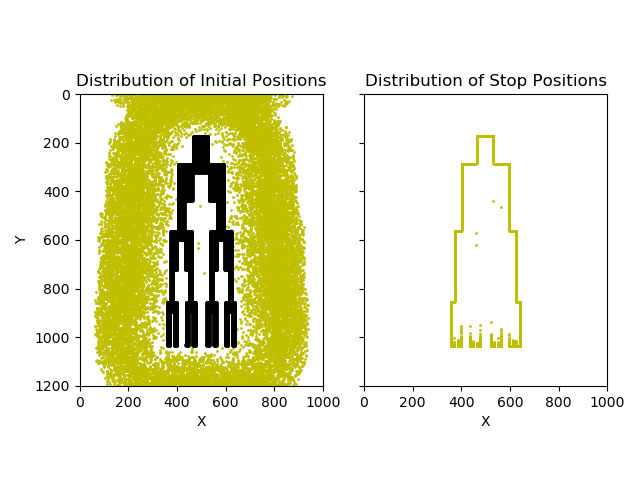
\includegraphics[width=\textwidth]{G_1_L_3_unwrap_disp_y_initial_pos_distribution.png}
          \caption{}
          \label{fig:G_1_L_3_disp_yellow_initial_pos_distribution}
        \end{subfigure}
        \caption{}
        \label{fig:G_1_L_3_steps_disp_yellow}
   \end{figure}




   \begin{figure}
        \centering
        \begin{subfigure}[b]{0.45\textwidth}
          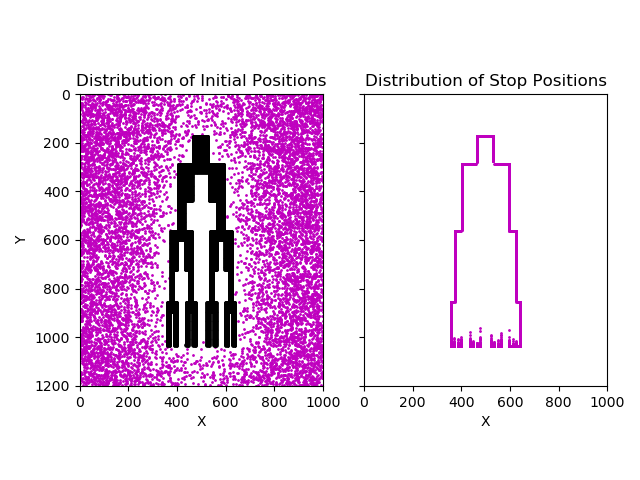
\includegraphics[width=\textwidth]{G_1_L_3_steps_m_initial_pos_distribution.png}
          \caption{}
          \label{fig:G_1_L_3_steps_pink_initial_pos_distribution}
        \end{subfigure}
        
        \begin{subfigure}[b]{0.45\textwidth}
          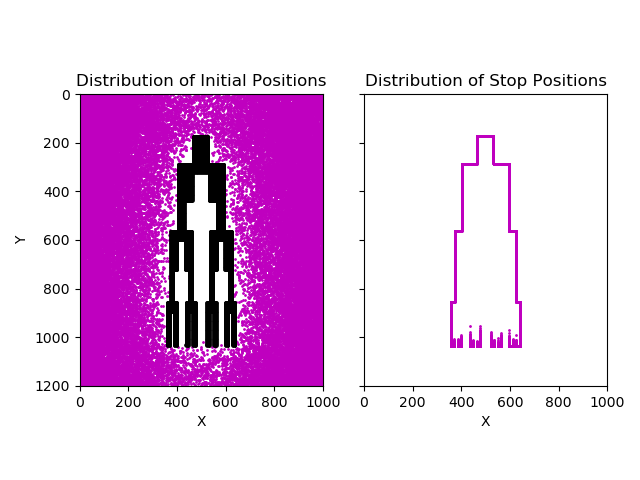
\includegraphics[width=\textwidth]{G_1_L_3_unwrap_disp_m_initial_pos_distribution.png}
          \caption{}
          \label{fig:G_1_L_3_disp_pink_initial_pos_distribution}
        \end{subfigure}
        \caption{}
        \label{fig:G_1_L_3_steps_pink_yellow}
   \end{figure}

   

   
   
\subsubsection{Comparison of Survival Curves}


  \begin{figure}
        \centering 
        \begin{subfigure}[b]{0.45\textwidth}
          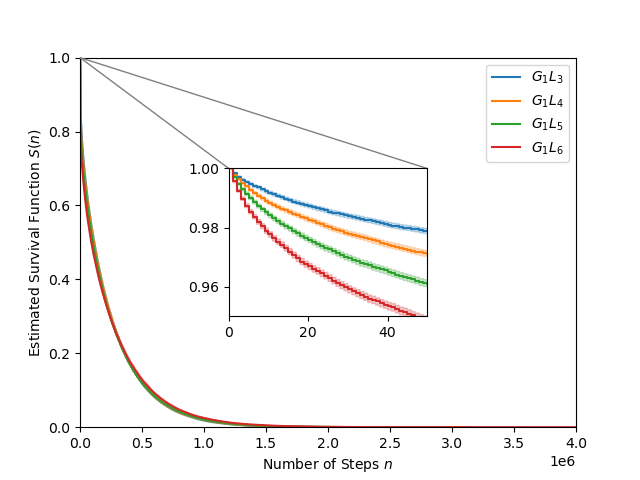
\includegraphics[width=\textwidth]{G_1_steps_sf.png}
          \caption{}
          \label{fig:sf_g1_branch_steps}
        \end{subfigure}
        \hfill
        \begin{subfigure}[b]{0.45\textwidth}
          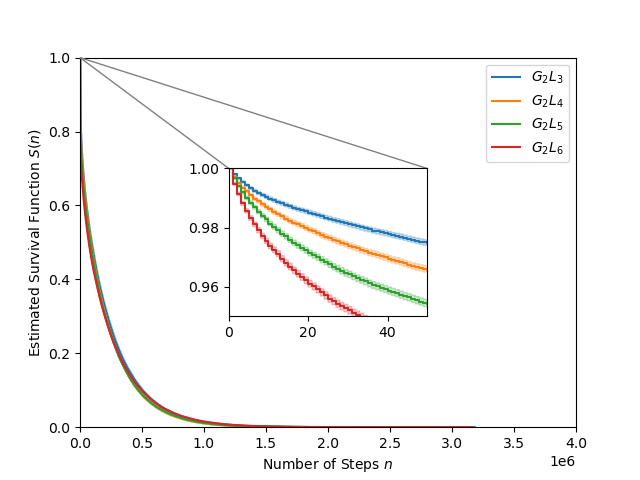
\includegraphics[width=\textwidth]{G_2_steps_sf.png}
          \caption{}
          \label{fig:sf_g2_branch_steps}
        \end{subfigure}
        \caption{(a) and (b) are survival functions for branching
          structures in $G_1$ and $G_2$, respectively. $n$ is the
          number of steps taken by the particle from the initial to
          the stop pixel in LRWs.}
        \label{fig:sf_branch_steps}
  \end{figure}

  \begin{figure}
        \centering
        \begin{subfigure}[b]{0.45\textwidth}
          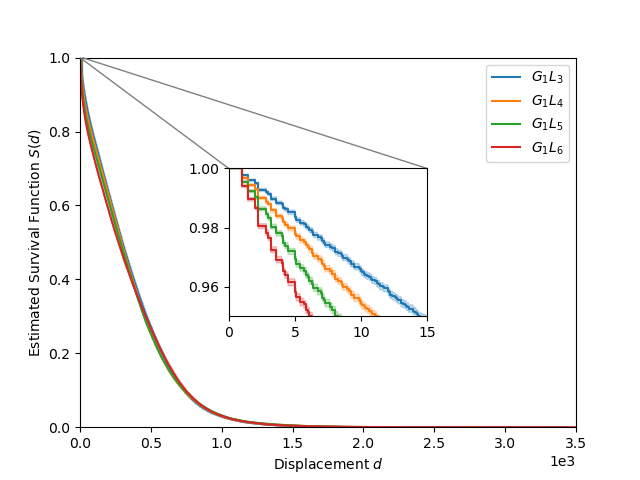
\includegraphics[width=\textwidth]{G_1_unwrap_disp_sf.png}
          \caption{}
          \label{fig:sf_g1_branch_disp}
        \end{subfigure}
        \hfill
        \begin{subfigure}[b]{0.45\textwidth}
          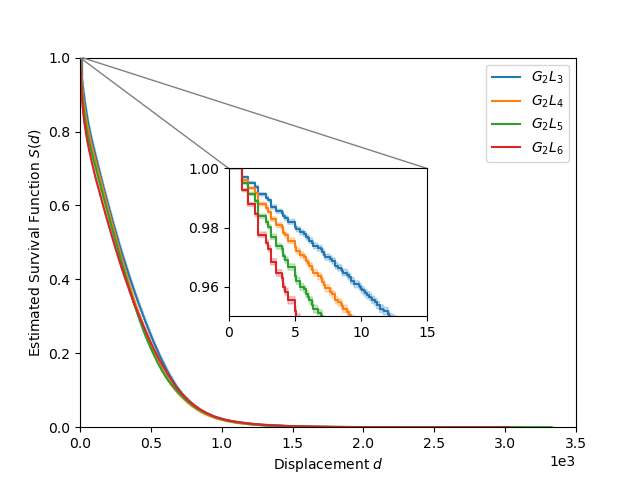
\includegraphics[width=\textwidth]{G_2_unwrap_disp_sf.png}
          \caption{}
          \label{fig:sf_g2_branch_disp}
        \end{subfigure}
        \caption{(a) and (b) are the estimated survival functions
          associated with particles' displacement in LRWs in $G_1$ and
          $G_2$, respectively.}
        \label{fig:sf_branch_disp}
  \end{figure}


  \begin{figure}
        \centering
        \begin{subfigure}[b]{0.45\textwidth}
          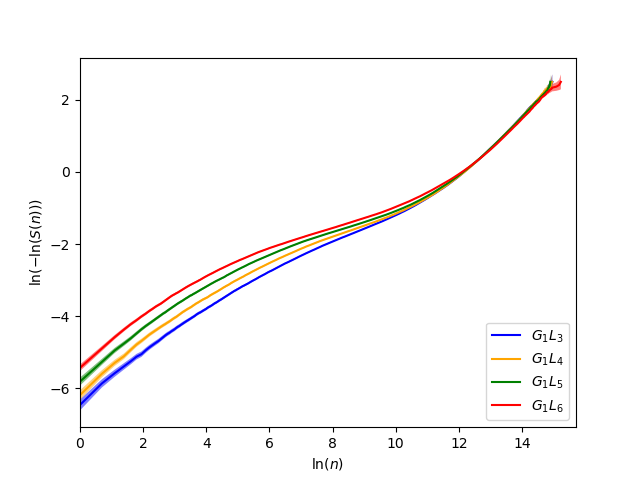
\includegraphics[width=\textwidth]{G_1_steps_check_ph.png}
          \caption{}
          \label{fig:g1_steps_check_ph}
        \end{subfigure}
        \hfill
        \begin{subfigure}[b]{0.45\textwidth}
          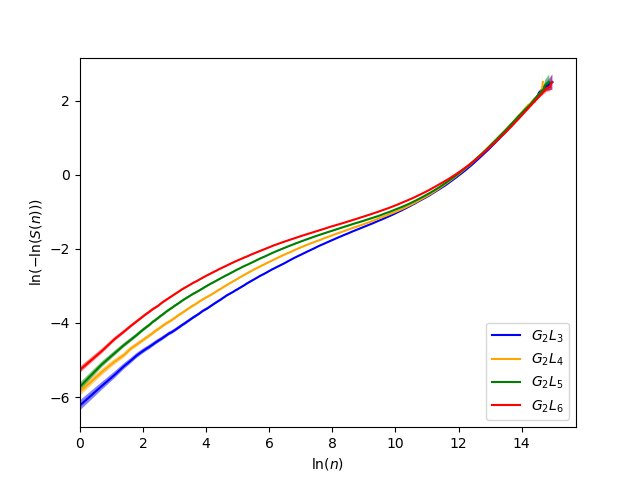
\includegraphics[width=\textwidth]{G_2_steps_check_ph.png}
          \caption{}
          \label{fig:g1_steps_check_ph}
        \end{subfigure}
        \caption{(a) and (b) are commonly used graphical techniques to
          check the proportional hazards (PH) assumption of survival data
          by finding the parallelism. The survival distributions do
          not support the PH assumption since the
          hazard ratio in both $G_1$ and $G_2$ is not always constant.}
        \label{fig:branch_steps_check_ph}
  \end{figure}


  \begin{figure}
        \centering
        \begin{subfigure}[b]{0.45\textwidth}
          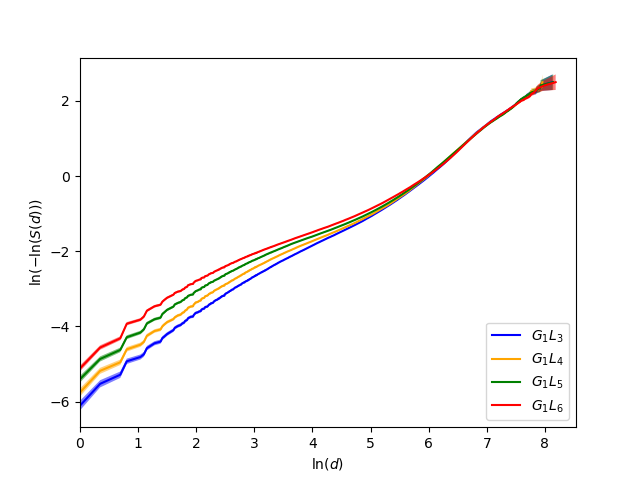
\includegraphics[width=\textwidth]{G_1_unwrap_disp_check_ph.png}
          \caption{}
          \label{fig:g1_disp_check_ph}
        \end{subfigure}
        \hfill
        \begin{subfigure}[b]{0.45\textwidth}
          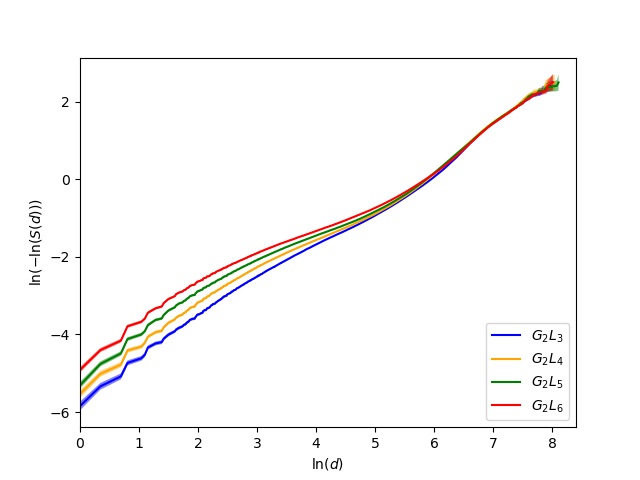
\includegraphics[width=\textwidth]{G_2_unwrap_disp_check_ph.png}
          \caption{}
          \label{fig:g1_disp_check_ph}
        \end{subfigure}
        \caption{}
        \label{fig:branch_disp_check_ph}
      \end{figure}



  \begin{table}
        \centering
        \begin{tabular}{llrrrr}
          \toprule
                       &             &         &  p &    &     \\
          \cmidrule{3-6}
                       &             & Log-rank & TW & GB & FH  \\
          \midrule
          $G_1$ $L_3$  & $G_1$ $L_4$  &  0.4393 &  0.0285 &  0.0005 &  0.0005     \\
                       & $G_1$ $L_5$  & 0.0 & 0.0 & 0.0 & 0.0    \\
                       & $G_1$ $L_6$  & 0.0 & 0.0 & 0.0 & 0.0      \\
          $G_1$ $L_4$  & $G_1$ $L_5$  & 0.0007 & 0.0 & 0.0 & 0.0      \\
                       & $G_1$ $L_6$  & 0.0002 & 0.0 & 0.0 & 0.0       \\
          $G_1$ $L_5$   & $G_1$ $L_6$ & 0.7223 &  0.0 & 0.0 & 0.0      \\
          \bottomrule
        \end{tabular}
        \caption{Two Sample Statistical Tests for $S(n)$ of $G_1$}
         \label{tab:g1_ingroup_tests_steps}
      \end{table}


      \begin{table}
        \centering
        \begin{tabular}{llrrrr}
          \toprule
                       &             &         &  p &    &     \\
          \cmidrule{3-6}
                       &             & Log-rank & TW & GB & FH  \\
          \midrule
          $G_2$ $L_3$  & $G_2$ $L_4$  &  0.0 &  0.0 &  0.0 &  0.0     \\
                       & $G_2$ $L_5$  & 0.0 & 0.0 & 0.0 & 0.0    \\
                       & $G_2$ $L_6$  & 0.0 & 0.0 & 0.0 & 0.0      \\
          $G_2$ $L_4$  & $G_2$ $L_5$  & 0.0016 & 0.0 & 0.0 & 0.0      \\
                       & $G_2$ $L_6$  & 0.0004 & 0.0 & 0.0 & 0.0       \\
          $G_2$ $L_5$   & $G_2$ $L_6$ & 0.7199 &  0.0 & 0.0 & 0.0      \\
          \bottomrule
        \end{tabular}
        \caption{Two Sample Statistical Tests for $S(n)$ of $G_2$}
        \label{tab:g2_ingroup_tests_steps}
      \end{table}


      
  \begin{table}
        \centering
        \begin{tabular}{llrrrr}
          \toprule
                       &             &         &  p &    &     \\
          \cmidrule{3-6}
                       &             & Logrank & TW & GB & FH  \\
          \midrule
          $G_1$ $L_3$  & $G_1$ $L_4$  &  0.0 &  0.0 &  0.0 &  0.0     \\
                       & $G_1$ $L_5$  & 0.0 & 0.0 & 0.0 & 0.0    \\
                       & $G_1$ $L_6$  & 0.0 & 0.0 & 0.0 & 0.0      \\
          $G_1$ $L_4$  & $G_1$ $L_5$  & 0.0072 & 0.0 & 0.0 & 0.0      \\
                       & $G_1$ $L_6$  & 0.0003 & 0.0 & 0.0 & 0.0       \\
          $G_1$ $L_5$   & $G_1$ $L_6$ & 0.2883 &  0.0 & 0.0 & 0.0      \\
          \bottomrule
        \end{tabular}
        \label{tab:g1_ingroup_tests_disp}
        \caption{Two Sample Statistical Tests for $S(d)$ of $G_1$}
      \end{table}


      \begin{table}
        \centering
        \begin{tabular}{llrrrr}
          \toprule
                       &             &         &  p &    &     \\
          \cmidrule{3-6}
                       &             & Logrank & TW & GB & FH  \\
          \midrule
          $G_2$ $L_3$  & $G_2$ $L_4$  &  0.0 &  0.0 &  0.0 &  0.0     \\
                       & $G_2$ $L_5$  & 0.0 & 0.0 & 0.0 & 0.0    \\
                       & $G_2$ $L_6$  & 0.0 & 0.0 & 0.0 & 0.0      \\
          $G_2$ $L_4$  & $G_2$ $L_5$  & 0.0001 & 0.0 & 0.0 & 0.0      \\
                       & $G_2$ $L_6$  & 0.0015 & 0.0 & 0.0 & 0.0       \\
          $G_2$ $L_5$   & $G_2$ $L_6$ & 0.7019 &  0.0 & 0.0 & 0.0      \\
          \bottomrule
        \end{tabular}
        \label{tab:g2_ingroup_tests_disp}
        \caption{Two Sample Statistical Tests for $S(d)$ of $G_2$}
      \end{table}

      



\subsubsubsection{Distance Matrices}




\subsubsubsection{Multidimenisonal Scaling}

